\chapter{Concurrent}\label{chap:concurrent}

本章及后章介绍数据库系统的事务处理机制，主要包括事务并发与恢复两部分。

\section{Transaction}

数据库是数据的共享资源池，当多个用户同时访问数据库，必然会带来一致性方面的问题。事务是一个抽象概念，它将用户的多个操作原子化，要么全部执行要么全部不执行。Jim Gray在\cite{Gray1992Transaction}一书中对事务处理的方案做了完备的介绍，他将事务总结为ACID四个方面的特性：
\begin{itemize}
    \item 原子性：事务的执行是原子性的；
    \item 一致性：事务执行前后，数据库的状态保持一致；
    \item 隔离性：事务与事务之间是隔离的，彼此不会干扰；
    \item 持久性：事务一旦提交，其对数据库状态的改变是永久的；
\end{itemize}

事务的原子性并不是说事务执行有多快，它要求事务的执行效果要么完全发生，要么完全不发生。计算机组成原理中，CPU原子操作是指CPU指令在执行过程中不会被中断。事务的隔离性是指事务与事务之间是隔离的，即一个事务的执行不会影响到其他事务的执行。操作系统中，进程之间通过地址空间隔离，事务的隔离要求在并发控制下协调运行。

ACID四个特性中，最难理解的是一致性，这个一致性本质上是用户的要求，但数据库作为一个独立的系统，如何满足外部的要求，需知用户的要求是千变万化的。一致性有两方面的要求：在用户侧，要求事务执行前后，用户对数据库的修改能够保证状态的一致；在这个前提下，数据库系统承诺，事务在并发或者出错场景下，依然能保证按用户的要求执行或者不执行。

事务是一个抽象概念，在数据库系统上，它对应于用户执行BEGIN/COMMIT的一个操作序列，这个操作序列由数据系统的会话层执行，它会调用执行引擎在事务引擎的控制下推进，并将结果写入存储引擎，将过程记录在日志中。在事务的执行过程中，它会占用不同的资源，包括索引、页面、记录、元数据等等，在事务执行完毕后，这些资源被释放。

并非仅有数据库系统才提供事务服务。在一个复杂系统中：一个web服务器后台挂着一个数据库系统，暴露各种http服务，用户通过Restful API调用这些服务。当用户开启一个事务，概念上，事务并不仅仅是数据库系统的一个操作序列，它的操作包括从客户发出的请求，web服务器的响应动作，底层数据的执行序列，涉及的对象包括客户端、web服务器、数据库。微软曾经引入Jim改造自己的分布式系统框架ActiveCOM，目的是在各种业务系统上提供事务服务。

\begin{exercise}
    事务不仅仅存在与数据库中，文件系统同样存在着类似的概念，考查Journal文件系统的设计，仔细甄别文件系统对事务的需求，对比它与数据库事务的异同。
\end{exercise}
\begin{exercise}
    自云计算兴起后，数据广泛的存储在分布式节点上，分布式存储系统如何保持数据的一致性？
\end{exercise}

\section{事务模型}

为了便于讲述事务的并发与恢复，需要先对数据库事务的操作抽象，这些抽象并不能完全反映数据的所有操作，但对理解事务并发与恢复的机制足够了。

\subsection{行模型}

关系型数据的数据模型是关系，关系由元组组成，事务对关系的操作是对元组的增删改查。所谓行模型，是将对元组的操作抽象为read/write两个操作，显然行的读写模型并不能涵盖元组上的所有操作，读写操作要求是可逆的。读的可逆操作，就是简单的drop掉读到的数据，写的可逆操作要求取消写入的元组，当事务恢复时，在恢复中会要求撤销以前的写操作。

\begin{exercise}
    对一个关系的操作包括增删改查CRUD，这些操作的逆操作是怎样的？
\end{exercise}

\begin{figure}[H]
    \centering
    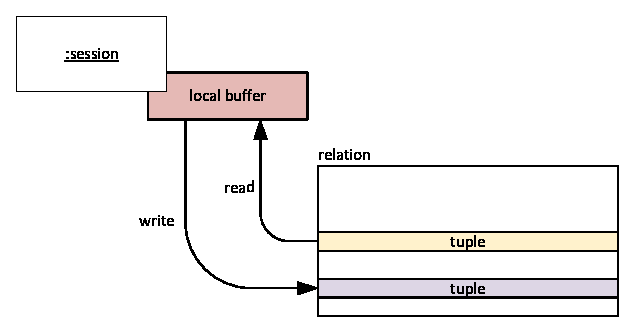
\includegraphics[width=0.8\linewidth]{handout/img/7-model.eps}
    \caption{行读写操作模型}\label{fig:7-model}
\end{figure}

\figurename\ref{fig:7-model}中，用户连接数据库，由会话代理用户执行SQL语句。假设一客户一会话，会话的本地缓冲对其它会话不可见。会话开启一个事务，先清空本地缓冲，然后按要求读元组，根据读到的元组在本地计算，最后将结果写入关系。写入关系的元组对其它事务不可见，只有当该事务提交后，事务的修改才可见。

有些事务实现不会在事务执行过程中去修改关系，而是在事务提交后，才去修改关系，这称为组提交策略。有些实现则在事务开启前不清空本地缓冲，这存在着风险，因为读到的数据可能不是最新，需要在修改元组或者提交事务时检查读到数据的有效性。在会话的实现中，除缓存元数据外，一般要求清晰地标定读集合与写集合，以便在提交事务时进行冲突检测。读集合与写集合除了保存元组数据外，还会保存元组的版本号。

会话代理执行SQL语句，不能假设事务的执行是线性的，事务的各种操作可能是并发的，例如一个事务可能会同时去读多个元组，或者一边读一边写。但在后文讲解中，一般都会假设事务的读写操作是顺序执行的，目的是为了便于表达，有助于理解事务的并发与恢复。总之，事务的行模型是一个读写操作的偏序模型，但讲解中用全序序列来表达。

$$
t=r(x)w(x)r(y)r(x)w(x)
$$

以上面的事务为例，事务先读$x$，然后写$x$，再读$y$和$x$，最后写$x$。这里例子里，事务对$x$元组写了两次，假设在事务可以在执行过程中写入关系，$x$对其它事务是不可见的；或者采用写提交策略，$x$的修改在会话本地，只有在事务提交后才会写入关系。后文在讨论事务并发中，一般会做如下假设，这个假设有助于简化讨论，并没有禁止事务实现对同一元组多次读写：

\begin{itemize}
    \item 在事务执行过程中，对同一元组不会读写两次；
    \item 在事务写入一个元组后，不会再读该元组；
\end{itemize}

行的读写操作一般由执行引擎实现，在并发控制中，锁方案要求控制对读写操作的推进，这要求并发控制会嵌入到执行引擎中。而在乐观并发控制中，读写操作的推进一般不受控制，事务在提交时会进行冲突检测。

\begin{exercise}
    如果采用偏序模型来描述事务执行的操作，它的表达应该是怎样的？
\end{exercise}
\begin{exercise}
    后文在介绍事务并发时，强加了不重复读写记录的假设。潜台词，事务的缺省隔离级别是多少？
\end{exercise}
\begin{exercise}
    在MVCC场景下，事务的执行是乐观的，在提交阶段才检查读写集合的冲突。我们前面假设会话执行SQL语句，会在本地保存记录的读集合与写集合，该如何实现？对比锁方案，能不能不在会话本地实现读写集合？
\end{exercise}

\subsection{树模型}

事务的操作抽象为行的读写，这种抽象是一种极致的简化，现实中，事务的操作远比行模型复杂得多。以一个银行转账事务为例，先从一个账户$a$提取1000元，然后将1000元存入另一个账户$b$。这两个操作要进一步分解为数据库的SQL语句，SQL语句然后被抽象为行的读写。

\begin{figure}[H]
    \centering
    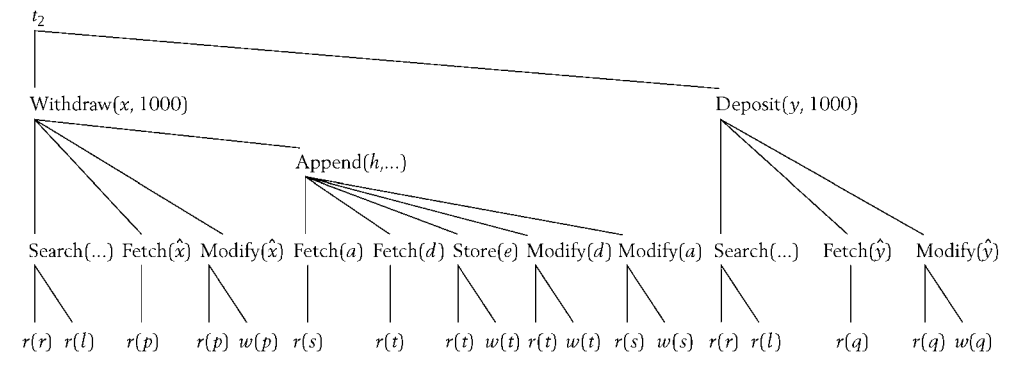
\includegraphics[width=\linewidth]{handout/img/7-tree.png}
    \caption{转账事务操作的树型模型}\label{fig:7-tree}
\end{figure}

在这个例子中，事务不仅是数据库上，而是全系统范围的操作序列。整个事务的执行被分解为多级，withdraw/deposit对应于账务的业务操作，Search/Fetch/Modify是数据库的操作，这些操作进一步分解为底层的行读写操作，所有操作按照树型组织。

树模型支持更丰富的语义，能够表达复杂的事务。树模型虽然分层，基础仍然是底层的行读写操作。以前面的withdraw为例，withdraw是一个业务操作，它会分解为数据库SQL语句，进一步分解为底层行模型。在业务层次，一般不会提供可逆操作，因为withdraw的分解并不一定是唯一的，withdraw的可逆性最终要依赖于底层的页模型来确保。

树模型的并发，也依赖底层页模型，底层页模型控制多个事务的推进。但是，并不是说树模型中某些操作不需要并发控制，有些中间操作是需要显式加入并发控制的。

数据库库内部的对象，并不仅限于数据元组，可能还有索引、页面、元数据等，在一个完整事务处理中，需要根据对象类型来处理并发与恢复，尤其是这些对象的逆操作实现。

\begin{exercise}
    一个聚集存储的页面上的操作有哪些？这些操作的逆操作如何实现？如果页面分裂，如何处理逆操作？
\end{exercise}
\begin{exercise}
    btree索引上的逆操作呢？
\end{exercise}

\subsection{版本模型}

将数据库存储的数据看成一个集合，每次事务提交对这个集合做更改。如果从用户需求来看，如果每次只访问最新的更新，整个数据集总是最新版本。这种模型下，事务并发一般采用锁方案，由两阶段锁2PL协议控制事务并发推进。锁方案下，事务更新的可见性按照标准分为4个隔离级别，这4种隔离级别的约束逐渐增高：

\begin{itemize}
    \item 读未提交（Read Uncommitted）：允许一个事务读取另一个事务未提交的数据，可能会导致脏读（Dirty Read），数据一致性差。
    \item 读已提交（Read Committed）：一个事务只能读取已提交事务的数据，避免了脏读，但可能会出现不可重复读（Non-repeatable Read）。
    \item 可重复读（Repeatable Read）：在同一事务中多次读取同一数据时，结果始终相同，避免了脏读和不可重复读，但可能会出现幻读（Phantom Read）。
    \item 可串行化（Serializable）：最高的隔离级别，强制事务串行执行，完全避免了脏读、不可重复读和幻读，但性能较低。
\end{itemize}

\begin{exercise}
    构造一个脏读的例子。
\end{exercise}
\begin{exercise}
    构造一个不可重复读的例子，在锁方案中，它出现的根本原因是什么？
\end{exercise}
\begin{exercise}
    构造一个幻读的例子，在锁方案中，它出现的根本原因是什么？
\end{exercise}

可串行化serializable与串行化serialized二者是存在根本区别的，可串行化目的是允许事务并发执行，串行化是将所有事务按照某种顺序串行执行。可串行化目的是提升系统吞吐量，执行的结果要等同于串行化执行，或者说，可串行化的目标是以并发的方式实现串行化的效果。

脏读、不可重复读、幻读的产生，都是由于是否加锁、是否加写锁、加读锁、对不存在项是否加锁的选择所致。要充分理解这4种隔离级别，需要从锁的方案出发。

如果用户允许数据库对象存在多个版本，但对象版本的增长要求为线性，此时可能会使得应用的性能得到显著提升。例如，一个公司要对上个月的销售情况做统计，这些统计操作并不需要最新的数据版本，允许读取一个历史版本即可。如果依赖于最新的数据，很可能会由于等待一个缓慢的事务，拖慢整个统计操作的完成时间。

\begin{figure}[H]
    \centering
    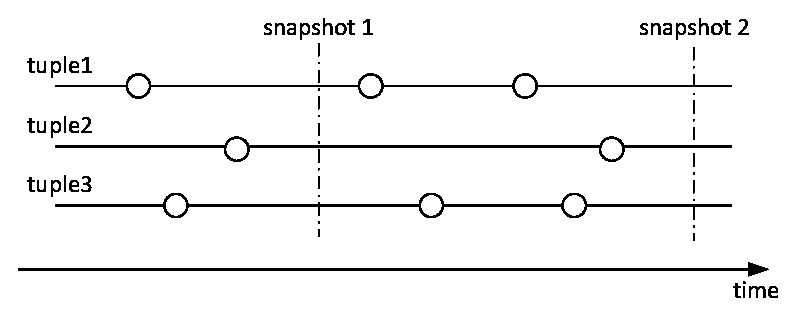
\includegraphics[width=0.8\linewidth]{handout/img/7-snapshot.eps}
    \caption{多版本事务}\label{fig:7-snapshot}
\end{figure}

如\figurename\ref{fig:7-snapshot}所示，每个元组有不同版本，根据时戳可以划分出不同的版本。对旧有版本的访问不会影响最新版本的更新，事务可以并发地读取不同版本的数据。

\begin{exercise}
    \figurename\ref{fig:7-snapshot}中展示的的多版本有统一的时钟，在分布式系统下，维护一个全局的物理时钟开销很大，如何利用因果关系在分布式节点上读取一个快照snapshot？参考\cite{lamport2019time}。
\end{exercise}

目前，数据库的多版本模型都是线性的，即对象可能存在多个版本，但是版本号是严格递增的。但有些应用中，版本的增加可能会出现分支，例如git版本控制系统。
\begin{exercise}
    线性版本系统，一般直接用时戳来标记版本。假设一个数据库的模板模型是非线性的，元组会出现分支版本，版本该如何表达？
\end{exercise}
\begin{exercise}
    假设有一个协同文档编辑系统，类似于wiki，它是一个非线性的版本系统吗？讨论一下。
\end{exercise}

\section{单版本并发}

在不同的版本模型下，事务并发控制的方案也不同。单版本模型下，事务读记录需要考虑该记录是否被修改或者将被修改，而多版本模型下，事务从某个snapshot上读数据，不会被阻塞。单版面模型需要考虑的资源共享问题更严格。

\begin{figure}[H]
    \centering
    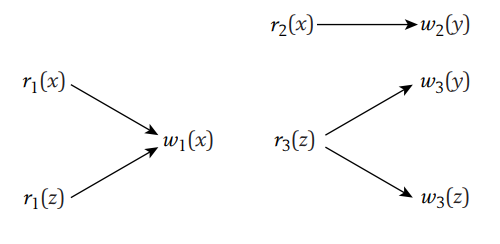
\includegraphics[width=0.6\linewidth]{handout/img/7-partial.png}
    \caption{三个事务}\label{fig:7-partial}
    \vspace{1em}
    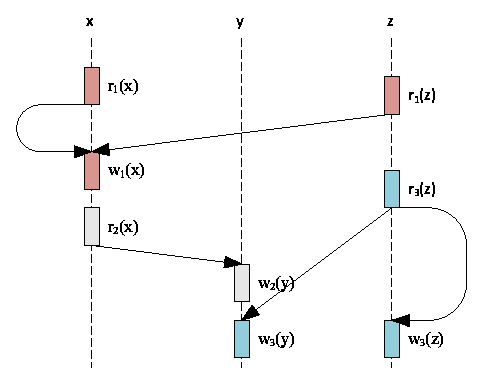
\includegraphics[width=0.7\linewidth]{handout/img/7-seq.eps}
    \caption{三个事务偏序执行}\label{fig:7-seq}
\end{figure}

\subsection{调度的正确性}

每个事务如果用偏序表达，多个事务并发，这些事务的r/w操作会交叠执行，将多个事务并发执行的偏序表达称为一个调度。在\figurename\ref{fig:7-partial}中有三个事务，它们的一种执行顺序如\figurename\ref{fig:7-seq}所示。我们要判定\figurename\ref{fig:7-seq}的执行过程是否符合事务的一致性要求，如果符合，这三个事务的并行执行就是合法的。

根据ACID的原则，一致性要求一个事务$t$执行前后数据库的状态必须是一致的。数据库的状态一致，在不同的场景下语义可能不同，行的读写操作并不能保证一致性，这种一致性是由用户保证的，数据库无法做出承诺。回到\figurename\ref{fig:7-partial}，可以断定单独执行$t_1, t_2, t_3$，数据库的状态是一致的，并且串行执行$t_1, t_2, t_3$三个事务，最终结果也是一致的。由此，判定\figurename\ref{fig:7-seq}是否合法，就需判定它是否等价于某个串行执行的结果。

\begin{exercise}
    假设有$n$个事务，它们串行执行的方案有多少种？
\end{exercise}
\begin{exercise}
    如果多个事务偏序并发，它们的并发方式比串行执行更多吗？是否每种偏序并发会对应于一种串行执行的结果？
\end{exercise}

\figurename\ref{fig:7-seq}的执行结果实际上等价于$t_1 > t_2 > t_3$，$r_3(z)$虽然在$t_2$前执行，但$z$的值与$t_2$是无关的，即使$r_3(z)$向下滑动到$w_2(y)$之后，结果仍然是相同的。

\begin{exercise}
    \figurename\ref{fig:7-seq}中，$w_3(z)$向上滑动到$w_2(y)$之前，是否是一致的？对数据库而言是一致的，但是数据库作为一个系统，它要向外暴露内部状态，在外部看来，$y,z$的数据更新发生交叠，这并不符合一致性预期。在单节点服务器上，要求事务的提交是顺序的，分布式数据库呢，是否也要求事务提交的全局顺序性？
\end{exercise}
\begin{exercise}
    \figurename\ref{fig:7-seq}中，如果将$w_2(y), w_3(y)$位置交换，是否是一致的？$w_1(x), r_2(x)$交换呢？
\end{exercise}

\subsection{调度的可串行化}

调度的可串行化serializable，是指一个调度等价于某个串行执行的结果。按照\cite{Weikum2001Transactional}，有多种等价定义，如语义可串行化、结果可串行化、视图可串行化、冲突可串行化等。其中，语义可串行化计算调度的语义，但如前所述，语义的定义与特定应用相关，数据库无法单独定义。结果可串行化只看调度完成后是否与某个串行调度等价，未考虑并发过程。视图可串行化VSR在结果可串行化的基础上，约束并发执行每一个操作都等价于某个串行调度，由于串行调度的数量庞大，是个NP难题。本文只从冲突可串行化开始介绍，更多的可串行化定义参考\cite{Weikum2001Transactional}。

\subsubsection*{冲突}

非形式化的，冲突是指同一资源上，两个事务间的操作间的关系。考虑行模型，记录上只有两种操作：读取和写入。$t_1$事务对资源$x$写入$w_1(x)$，$t_2$事务对资源$x$读取$r_2(x)$，如果$w_1(x)$在$r_2(x)$之前执行，$t_1$和$t_2$是冲突的。行模型中，只有$r_1(x)r_2(x)$操作是不冲突的，其余写操作都会引起冲突。

冲突发生，实际上规定了事务间的执行顺序，以$w_1(x)r_2(x)$为例，它要求$t_1 > t_2$。利用从冲突得到的事务间偏序关系，可以构造后面的冲突图，如果图上存在环，则可以判定调度不可串行化，这是引入冲突概念的目的。

给定一个调度$s$，找出在同一资源上的所有两两冲突关系，这些两两冲突构成了这个调度的冲突集，利用这个冲突集可以构造后文的冲突图。当两个调度的冲突集相同，称这两个调度等价。
$$
s=w_1(x)r_2(x)w_2(y)r_1(y)w_1(y)w_3(x)w_3(y)c_1a_2
$$
上式中，调度$s$的冲突集如下。在计算冲突集时，当遇到取消事务时，简单地将该事务的所有操作忽略掉，例如上式中$t_2$被取消，$r_2(x)$和$w_2(y)$都被忽略。
$$
conf(s) = \{ (w_1(x),w_3(x)), (r_1(y), w_3(y)), (w_1(y), w_3(y)) \}
$$

\begin{exercise}
    两个调度$s, s'$是否等价？
    $$
    s=r_1(x)r_1(y)w_2(x)w_1(y)r_2(z)w_1(x)w_2(y)
    $$
    $$
    s'=r_1(y)r_1(x)w_1(y)w_2(x)w_1(x)r_2(z)w_2(y)
    $$
\end{exercise}

\subsubsection*{冲突可串行化CSR}

按照可串行化正确性的规定，冲突可串行化定义为：如果一个调度与某个串行调度等价，称这个调度是冲突可串行化的。举例而言，
$$
r_1(x)r_2(x)r_1(z)w_1(x)w_2(y)r_3(z)w_3(y)c_1c_2w_3(z)c_3
$$
上式的冲突集为
$$
\{ (r_2(x), w_1(x)), (w_2(y), w_3(y)), (r_1(z),w_3(z))\}
$$
这个冲突集等价于$t_2 < t_1 < t_3$，如果刨除调度尾部的提交动作，这个调度是冲突可串行化的。注意到上式中提交顺序$c_1c_2c_3$与等价串行化序列并不相符，后文将定义更严格的提交保序冲突可串行化。

再举一个例子，$r_2(y)w_1(y)w_1(x)c_1w_2(x)c_2$的冲突集为$\{(r_2(y),w_1(y)),(w_1(x),w_2(x))\}$，冲突集的两项是矛盾的，没有串行化序列与之对应。从这个例子，进一步引申出冲突图的概念，冲突图是一个有向图，图中每个节点对应于一个节点，冲突关系规定了两个节点的先后顺序，从前一个节点指向后一个几点。要判定一个调度是否合法，只需保证冲突图无环。

\begin{figure}[H]
    \centering
    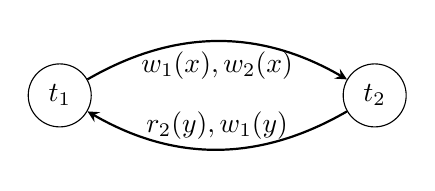
\begin{tikzpicture}[node distance=4cm, auto, >=stealth]
        % 事务节点
        \node[draw, circle, minimum size=0.8cm] (t1) {$t_1$};
        \node[draw, circle, minimum size=0.8cm, right of=t1] (t2) {$t_2$};

        % 冲突边
        \draw[->, thick] (t2) to [bend left=30] node[above] {$r_2(y), w_1(y)$} (t1);
        \draw[->, thick] (t1) to [bend left=30] node[below] {$w_1(x), w_2(x)$} (t2);
    \end{tikzpicture}
    \caption{冲突集$\{(r_2(y),w_1(y)),(w_1(x),w_2(x))\}$对应的冲突图}
    \label{fig:conflict-graph}
\end{figure}

\subsubsection*{提交保序可串行化COP}

冲突可串行化CSR没有考虑到提交顺序，提交顺序保持冲突可串行化Commit-Order Preserving CSR(COP)在CSR基础上，要求提交顺序与CSR串行化顺序一致。
$$
s_1 = w_1(x)r_2(x)c_2w_3(y)c_3w_1(y)c_1
$$
$s_1$是CSR，等价串行化调度为$t_3t_1t_2$，按照COP定义，事务提交顺序是$t_2t_3t_1$。

$$
s_2 = w_3(y)c_3w_1(x)r_2(x)w_1(y)c_1c_2
$$
$s_2$是CSR，等价串行化调度为$t_3t_1t_2$。提交顺序是$c_3c_2c_1$，$s_2$是COP。

\begin{figure}[H]
    \centering
    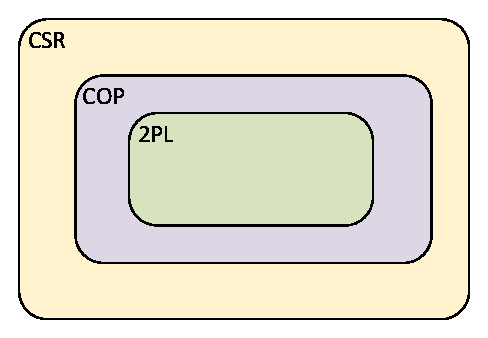
\includegraphics[width=0.4\linewidth]{handout/img/7-cop.eps}
    \caption{CSR、COP、2PL间的关系}\label{fig:7-cop}
\end{figure}

\begin{exercise}
计算下式的冲突集，等价串行化调度，画出冲突图，是否COP。
$$
s = r_1(y)r_3(w)r_2(y)w_1(y)w_1(x)w_2(x)w_2(z)w_3(x)c_1c_2
$$
\end{exercise}

\subsection{锁方案}

COP是大多数基于锁方案的事务并发的理论基础。冲突发生，实际上规定了两个事务间的先后顺序，确定了CSR对应的串行化调度，当提交顺序与CSR串行化顺序一致时，调度就是COP。事务提交顺序与CSR串行化顺序不一致，会破坏事务的可见性。但事务何时提交完全由用户确定，事务引擎实现只能退而求其次，禁止所有冲突的发生。也就是说，事务访问资源，如果发生冲突，会阻止事务推进，阻塞事务，这种机制正好用锁来实现。

\begin{exercise}
    冲突可串行化的接受调度为COP，由于不确定事务间的提交顺序，只能采用锁方案。锁方案采用后文的2PL协议，接受的调度集合是COP的子集。假设已知事务及其提交顺序，有没有可能实现COP？
\end{exercise}

回顾一下事务并发的场景，会话代理执行SQL语句，这些语句会读写底层记录。为了尽可能提升系统吞吐量，系统需要支持多事务并发。采用锁来实现冲突检测，当事务访问资源，检测是否发生冲突，如果发生冲突，阻塞事务执行，等待其他事务释放锁。当其它事务提交，是否资源上的锁，锁会通知事务线程继续执行。

事务的推进由锁控制，它的逻辑是嵌入到行模型的读写操作中，这不太友好，好消息是树模型的事务虽然复杂，我们只需要关注底层行模型的实现即可。

\subsubsection*{事务状态机}

在数据库中，会话代理用户执行SQL语句，一个会话对应一个客户。会话是活动对象，通常用线程或者进程来表示。当会话开启一个事务，事务进入Running状态，访问资源发生冲突，事务被阻塞。事务完成后，进入提交状态，这是事务的终态。当事务被取消，事务会重启，重新开始，如\figurename\ref{fig:7-states}。

\begin{figure}[H]
    \centering
    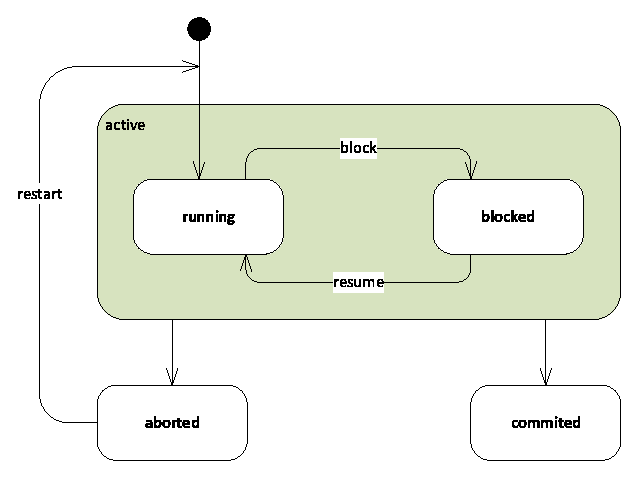
\includegraphics[width=0.8\linewidth]{handout/img/7-states.eps}
    \caption{事务状态机}\label{fig:7-states}
\end{figure}

\subsubsection*{锁表}

锁方案在内存中建立一个锁表，每行对应于一把锁。当事务访问记录时，在锁表中创建记录对应的锁，然后对记录加读锁或写锁。如果加锁成功，事务继续执行；如果加锁失败，事务阻塞，等待其他事务释放锁。

\begin{exercise}
    锁方案中，一条记录一把锁，可以在记录上建立锁吗？
\end{exercise}

由于行数会很多，而事务访问的资源，在某些场景下并不一定很多，所以锁表里的锁是按需创建的。但在记录中内嵌锁，并不是不可行，只是在传统关系型数据库中，系统崩溃，意味着接受的未完成事务会被放弃，持久化锁没有意义。而在分布式系统中，系统运行的容错模型要求$7 \times 24$不间断，单个节点崩溃意味着锁的丢失，其余节点重启服务，会导致事务推进错误，所以在Percolator\cite{peng2010large}中锁被持久化到kv存储中。

锁表包含锁，事务访问资源，会先进入锁表查看资源是否有锁，如果没有则创建，然后加锁。如果有锁，则访问该锁。目前的锁表方案是hash+btree，利用hash实现对点加锁，利用btree处理范围锁。

\begin{exercise}
    能否利用区间树interval tree来设计锁表，支持点、范围加锁？
\end{exercise}

\subsubsection*{锁的设计}

锁的基本结构，如\ref{fig:7-lock}所示，每个记录对应于一把锁，锁的状态包括未加锁、读锁、写锁。当事务访问记录时，在锁表中创建记录对应的锁，然后对记录加读锁或写锁。如果加锁成功，事务继续执行；如果加锁失败，事务阻塞，进入等待状态，等待其他事务释放锁。

\begin{figure}[H]
    \centering
    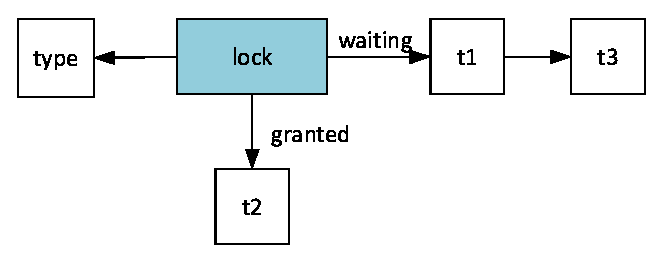
\includegraphics[width=0.6\linewidth]{handout/img/7-lock.eps}
    \caption{锁的设计}\label{fig:7-lock}
\end{figure}

将读锁标记为S，写锁标记为X，根据冲突检测规则，S锁与S锁不冲突，S锁与X锁冲突，X锁与X锁冲突，有\figurename\ref{fig:7-lock}的相容性矩阵。

\begin{table}[H]
    \centering
    \caption{S锁和X锁的相容性矩阵}\label{tab:lock}
    \begin{tabular}{ccc}
        \toprule
        \textbf{请求类型} & \textbf{已加S锁} & \textbf{已加X锁} \\
        \midrule
        \textbf{S锁} & $\checkmark$ & $\times$ \\
        \textbf{X锁} & $\times$ & $\times$ \\
        \bottomrule
    \end{tabular}
\end{table}

事务在执行过程中，开始可能并不知道是否要对一行加锁，后面才决定写该行。此时事务持有S锁，如果没有其它事务同时持有这个S锁，可以安全地升级为X锁。这里的问题是，如果该S锁被多个事务持有，升级为X锁会导致其他事务阻塞，该如何处理？一般的方案是，将该锁标记为待升级，待升级标志指向希望升级的事务。进一步，当多个持有S锁的事务同时希望升级，会发生死锁。

行模型是一种简单的模型，数据库中除了行外，还包括索引、页等结构，事务对这些结构的访问，要复杂一些。以SELECT FROM WHERE语句为例，事务需要先查询btree索引，找到符合条件的记录，然后对这些记录加S锁。多数数据库实现中，将btree看成是内部数据结构，以latch方式加锁，latch不同于lock，它用完后立即释放。innodb实现中，先对btree加latch，找到记录后，对记录加S锁，释放latch，latch不遵循后面的2PL协议。考虑到事务正在读该表的某行，innodb可能会对该表加一个意向锁，禁止删除该表。

从上面的讨论中，可以看到，数据库中锁的设计非常精妙细微，一般分为表锁和行锁，表锁的设计需要根据细微的语义设计兼容性矩阵。

\begin{exercise}
    检查innodb与PostgreSQL中表锁的设计，体会这些锁的设计意图。
\end{exercise}

\subsubsection*{2PL协议}

事务对资源的访问一般遵循两阶段2PL协议，获取锁后，事务会持续访问资源，直到提交或回滚。2PL协议是说事务对锁的持有和释放是有序的，先获取锁然后再释放，观察\figurename\ref{fig:7-2pl}，事务的资源持有呈现为单峰。注意，单峰的衰减实际发生在提交或回滚阶段，设想一下，如果在提交前释放锁，意味着放弃对该资源的冲突检测。

采用2PL协议实现的调度器，它接受的调度集合是COP的子集，如\figurename\ref{fig:7-cop}。

\begin{figure}[H]
    \centering
    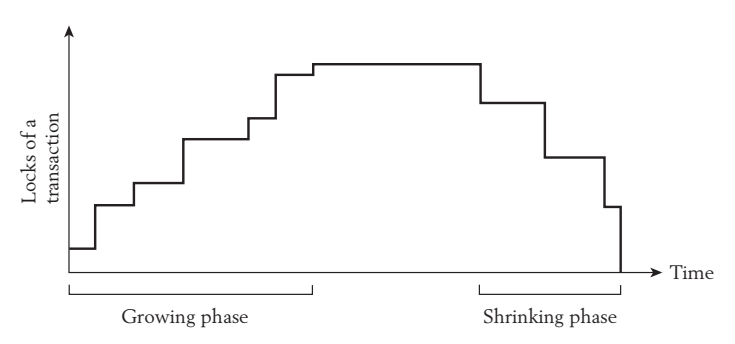
\includegraphics[width=0.8\linewidth]{handout/img/7-2pl.png}
    \caption{2PL协议}\label{fig:7-2pl}
\end{figure}

\begin{exercise}
    在2PL协议中，在提交前先释放读锁是否可行？如果不可行，举出反例。
\end{exercise}

\subsubsection*{死锁检测}

数据库内部加表锁和行锁后，可能会导致死锁的发生，死锁是多个事务彼此持有资源，等待对方释放锁，导致所有事务无法推进。操作系统课程中，关于死锁部分的内容包括死锁的检测和避免。数据库中采用类似的方案，一般会维护一个全局等待图。

在等待图waiting graph中，每个事务对应于一个节点v，当事务$t_1$等待某个锁，该锁被其它事务$t_2$持有，会画一条边$t_1 \rightarrow t_2$，从$t_1$出发，沿着这些边遍历，如果形成环，则表面存在死锁，对应着资源的彼此持有。实现中，这个等待图比较大，一般是在事务阻塞时启动一个定时器，超时后从该事务出发检测死锁。

当检测到死锁，会以某个标准选出环上的一个事务来牺牲，打破等待环，被选中的事务回滚重试。

\begin{exercise}
    事务由会话发起，构思一下这个等待图如何设计与实现。每个节点用vector容纳出边，对应于一个会话，会话有指针指向这个vector，出边需要描述lock。然后带入前述的多事务升级共享锁导致的死锁，看看这个方案需要补充什么。
\end{exercise}

\subsubsection*{死锁预防}

目前的死锁预防策略主要是基于时戳，假设每个事务启动都带有一个初始时戳，在此前提下，有如下两种方案：
\begin{itemize}
    \item wait-die：一个事务请求锁时，如果锁被其它事务持有，且该事务的时戳较大，那么该事务会等待；如果锁被其它事务持有，且该事务的时戳较小，那么该事务会回滚。也就是说，事务只会等待更年轻的事务，否则会回滚。
    \item wound-wait：一个事务请求锁时，如果锁被其它事务持有，且该事务的时戳较小，那么该事务会等待；如果锁被其它事务持有，且该事务的时戳较大，那么该事务会尝试杀死持有该锁的事务。也就是说，事务只会等待更老的事务，否则会杀死年轻事务。
\end{itemize}

现代主流数据库较少采用死锁预防，而更倾向于死锁检测，原因是死锁预防方案会减少可接受的调度集合，而死锁检测方案不会。

\section{多版本并发}

这本讲义中，关于锁的内容主要参考了\cite{Weikum2001Transactional}，可惜的是，mvcc方案真正成熟是在2009年之后。TIS\cite{Weikum2001Transactional}对多版本并发的描述较为简略，并且个人认为这部分的理论分析是错误的。

本节的内容主要参考了\cite{berenson1995critique, fekete2005making, cahill2009serializable}。\cite{berenson1995critique}指出SQL-92标准中的4种隔离级别用几种异常来划分，并不能正确区分一些某些异常，并提出一种基于多版本的snapshot isolation隔离级别。\cite{fekete2005making}形式化定义了 SI 的语义模型，指出write-skew是 SI 的根本缺陷。\cite{cahill2009serializable}在SI基础上，自动检查并阻断写偏序write-skew异常的发生，从而实现可串行化。

\subsection{一些基本前提}

在讨论多版本并发前，需要明确一些基本前提。多版本事务模型是线性的，对象按照线性版本递增。每个事务都带有两个时戳，一个是启动时戳，一个是提交时戳\cite{berenson1995critique}，一般用启动时戳来标记事务。启动时戳是事务执行BEGIN语句分配的时戳，提交时戳是事务执行COMMIT语句分配的时戳，时戳的分配是全局递增的，这在分布式场景下要求过于严格。

\begin{exercise}
    查阅google spanner的论文，了解truetime的设计目标与方案。
\end{exercise}

事务使用启动时戳读取数据，在会话本地计算，本地缓冲临时版本，使用组提交策略，这避免了脏读。事务执行COMMIT命令，先用latch锁住所有写入对象，然后用会话局部版本更新数据，提交后释放latch。

\begin{exercise}
    不用latch用锁行不行？可以的，这里用latch主要是因为SI隔离级别实现是无锁的。在\cite{cahill2009serializable}中，SSI可串行化的调度器使用了锁，参考一下该论文。
\end{exercise}

事务读取的版本是启动时戳之前的最近版本，启动时戳实际上对应了一个快照snapshot，加上组提交策略，事务天然避免了脏读和不可重复读，这对应了一个称为snapshot isolation的隔离级别\cite{berenson1995critique}。SI隔离级别并不等同于可重复读隔离级别，因为它并没有杜绝幻读，同时具有写偏write-skew异常。不能说SI与RR隔离级别哪个更高，基于锁的RR隔离级别与SI不完全等同。

\begin{exercise}
    参考一下\cite{berenson1995critique}，指出SI隔离级别与RR隔离级别为什么不同。
\end{exercise}

mvcc讨论的基线是SI隔离级别，因为SI基本非常吸引人，它天然高于读未提交RU和读已提交RC隔离级别，并且没有在对象上加锁，这使得它具有更好的性能。

\subsection{SI}

SI隔离级别的实现非常容易，事务读取启动时戳的快照，在提交时刻检查是否存在被提交时戳更高的版本即可。多个事务同时提交，latch竞争采用first-write-wins策略，即先提交的事务获得latch，后提交的事务等待。

\begin{figure}[H]
    \centering
    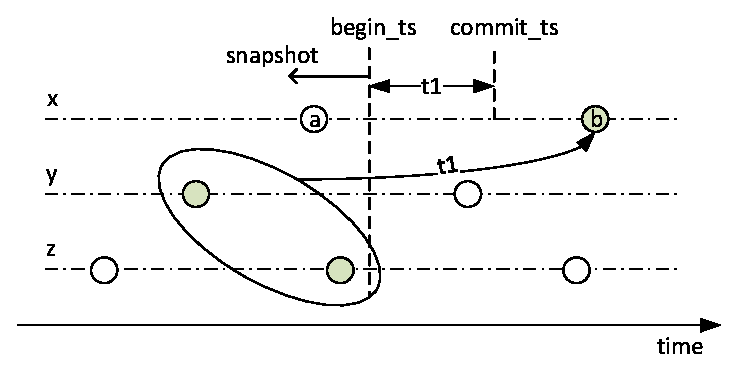
\includegraphics[width=0.8\linewidth]{handout/img/7-version.eps}
    \caption{提交写入过程}\label{fig:7-version}
\end{figure}

这里需要对提交时戳做一个更细部的说明，如\figurename\ref{fig:7-version}，事务读取启动时戳快照上的版本$y, z$，然后更新$x$。采用组提交策略，写入$x_b$版本时，使用提交时戳。事务的提交是需要时间的，对$x$的写入并不会发生在提交时戳的当下，而是需要拖后一段时间。如果latch加锁不成功，还可能导致事务的回滚。

\begin{exercise}
    mvcc中，是否需要检查死锁？如何防止latch的死锁？
\end{exercise}

\subsection{版本冲突}

令人惊讶的是，mvcc的相关理论与技术在2009年前后才成熟，而其时已进入了云计算与大数据时代。在此之前，Oracle 9.2宣称的SERIALIABLE隔离级别，实际上是SI隔离级别\cite{fekete2005making}。

与单版本并发类似，多版本并发的正确性准则仍然是——并发调度是否等价于多个事务的串行化调度。单版本上要求冲突集等价，多版本上仍然是要求冲突集等价，但是多版本上的冲突定义有变化，甚至可以不称之为冲突。单版本的冲突表现为同一行上操作间不相容，一个事务在改变数据，另一个事务依赖于旧值。而在多版本上，读写分别落在不同的版本上，写不会改变旧值，新版本的增加带来的问题更多的要从因果逻辑上看。

下面分析多版本的冲突，设有一个对象$x$，它的版本为$x_1, x_2, x_3, \ldots$，每个版本都有一个时戳$t_1, t_2, t_3, \ldots$。在讨论冲突时，需要讨论相邻版本间的冲突，即$x_1$与$x_2$、$x_2$与$x_3$等版本之间的冲突。跨版本间不存在冲突，例如$x_1$与$x_3$之间不存在冲突。同时，不同数据$x,y$上的操作间不存在冲突。

\subsubsection*{rr}

虽然由于两个事务$t_1, t_2$的启动时戳不同，对应于不同的快照，两个事务读同一个版本的对象，并不冲突。如\figurename\ref{fig:7-rr1}，两个事务启动时戳不同，对应于不同的快照，但读同一个版本的$x$，它们并不冲突。由于没有冲突，我们无法根据对该版本的读操作推测两个事务的串行化先后顺序。

对于读操作而言，无需讨论两个事务读不同版本的情况，如$r_1(x_1)r_2(x_2)$。原因在于，事务读到的版本不同，必然有某个事务写入了新版本，本质上是读写rw/wr关系，而不是不同版本的读读关系。

\begin{figure}[H]
    \centering
    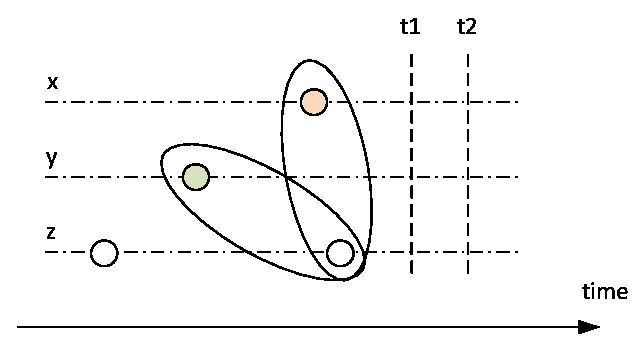
\includegraphics[width=0.6\linewidth]{handout/img/7-rr1.eps}
    \caption{两个事务读同一版本}\label{fig:7-rr1}
\end{figure}

在\figurename\ref{fig:7-rr2}中，事务$t_1$读取$x_a$，事务$t_2$读取$x_b$，但在$t_2$之前一定有一个$t_3$事务写入了$x_b$版本。

\begin{figure}[H]
    \centering
    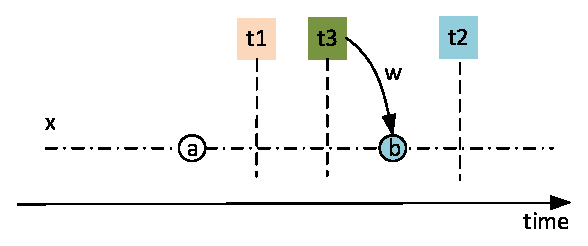
\includegraphics[width=0.6\linewidth]{handout/img/7-rr2.eps}
    \caption{两个事务读不同版本}\label{fig:7-rr2}
\end{figure}

\subsubsection*{wr}

一个事务写入新版本，另一个事务读取该版本，$w_1(x_1)r_2(x_1)$，两个事务操作在同一版本上。考查这种wr关系，它规定了写事务必须先写入，才能被读事务读取。

\begin{figure}[H]
    \centering
    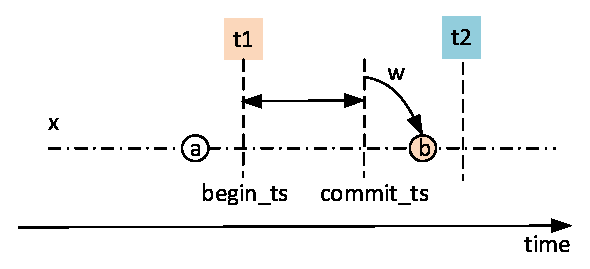
\includegraphics[width=0.6\linewidth]{handout/img/7-wr.eps}
    \caption{写读wr冲突}\label{fig:7-wr}
\end{figure}

在组提交策略下，$w_1(x)$写入动作在提交前做出，意味着$t_1$的提交时戳必然小于$t_2$的启动时戳，否则$w_1(x)$对$t_2$不可见，如\figurename\ref{fig:7-wr}。因此wr冲突的两个事务不会其实不会出现并发执行，$t_1, t_2$本身是串行执行的，在后文中wr不被认为是一种冲突。由于采用组提交策略，在表示调度时，一个事务写入新版本，后面会紧跟着提交动作。

\subsubsection*{rw}

一个事务读取老版本，另一个事务写入新版本，$r_1(x_0)w_2(x_2)$。两个事务操作在不同版本上，这是一个读写冲突，如\figurename\ref{fig:7-rw}。
\begin{figure}[H]
    \centering
    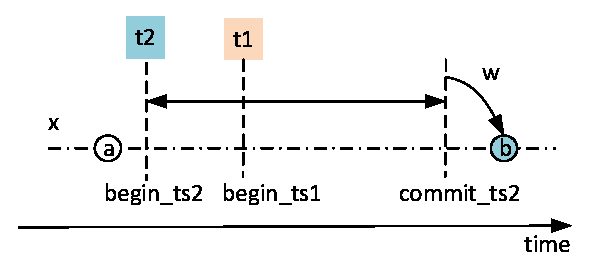
\includegraphics[width=0.6\linewidth]{handout/img/7-rw.eps}
    \caption{读写rw冲突}\label{fig:7-rw}
\end{figure}

在\figurename\ref{fig:7-rw}中，$t_2$写入版本$x_b$，$t_1$读取版本$x_a$，$x_b$对$t_1$不可见，说明begin\_ts1 < commit\_ts2。

对rw的分析可以有两种方法，一种是观察并发是否相对于串行化调度引入了新的冲突，另一种是根据rw的冲突含义，分析是否会产生因果矛盾。

将一个事务看成一个函数，读取作为输入，写入作为输出，输出依赖于输入。这个假设中，可能某个输出只依赖于部分输入，但这是用户所知，作为数据库而言，只能假设一个输出依赖于所有输入。

将事务的所有读取行记作读集合rset，事务的所有写入行记作wset。\figurename\ref{fig:7-rw}中的读写冲突实际上是两个事务的读写集合出现了版本交叠，如\figurename\ref{fig:7-wset}所示。

\begin{figure}[H]
    \centering
    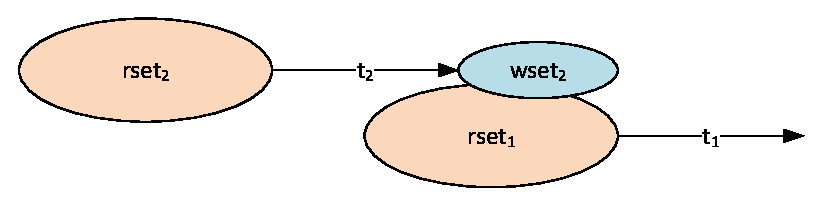
\includegraphics[width=0.8\linewidth]{handout/img/7-wset.eps}
    \caption{两个事务读写集合交叠}\label{fig:7-wset}
\end{figure}

$r_1(x_0)w_2(x_2)$这两个作用在$x$对象上的操作本身并不冲突，它们是两个版本。但问题是每个事务从rset $\rightarrow$ wset，这是一个因果关系，两个事务在这个前提下有可能会产生因果矛盾。


两个事务的等价串行化调度为$t_1t_2$或者$t_2t_1$，rw冲突下有$rset_1 \cap wset_2 \neq \emptyset$，先考查$t_1t_2$串行化调度，然后考查$t_2t_1$串行化调度：

\begin{itemize}
    \item $t_1t_2$：
    \begin{itemize}
        \item \figurename\ref{fig:7-rw2}中(a)所示，$t_1$先执行$t_2$后执行，冲突集中可能会包含一些wr冲突，但冲突并不意味着不可串行化。
        \item 将$t_1$向右滑动，如果$wset_1 \cap rset_2 = \emptyset$，冲突集没有变化，但不能就此判断是否可串行化。因为$t_1$的wset有可能与其它事务的rset交叠，导致新的冲突。
        \item \figurename\ref{fig:7-rw2}中(b)所示，如果$wset_1 \cap rset_2 \neq \emptyset$，并且$wset_1$对$t_2$不可见，这里有新的冲突$r_2(y_0)w_1(y_1)$。逻辑上，$t_2$的输出部分依赖于$t_1$，$t_1$的输出部分依赖于$t_2$，而(b)中这些输出又相互不可见，是矛盾的。
        \item 当$t_1$继续向右滑动，需要考虑$wset_1 \cap wset_2$，这是ww冲突。
    \end{itemize}
\end{itemize}

\begin{figure}[H]
    \centering
    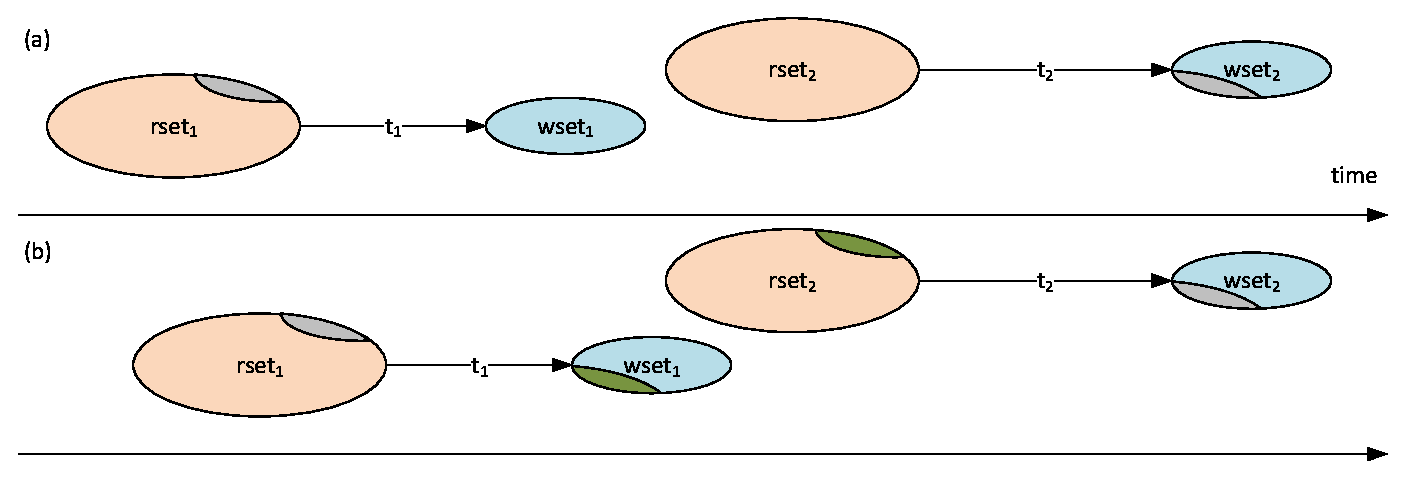
\includegraphics[width=\linewidth]{handout/img/7-rw2.eps}
    \caption{rw等价于$t_1t_2$冲突集}\label{fig:7-rw2}
\end{figure}

\begin{exercise}
    考查$t_2t_1$的等价冲突集。
\end{exercise}

rw读旧版本写新版本，两个事务分别在两个版本上操作，这两个操作之间其实没有冲突，关键是按照因果关系，事务间可能因为rset与wset之间的交集形成彼此依赖的循环关系。

\subsubsection*{ww}

两个事务写同一个对象，$w_1(x_1)w_2(x_2)$，这两个事务操作在不同版本上，两个操作本身没有冲突。在\figurename\ref{fig:7-ww}中，$t_1$先执行$t_2$后执行，冲突集中可能会包含一些ww冲突。在后文分析中，ww之间存在的问题实际上被转化为rw冲突。

\begin{figure}[H]
    \centering
    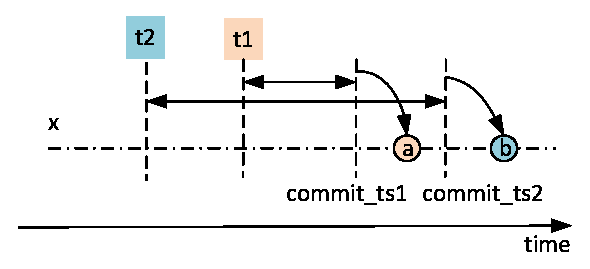
\includegraphics[width=0.6\linewidth]{handout/img/7-ww.eps}
    \caption{写写ww冲突}\label{fig:7-ww}
\end{figure}

两个事务$t_1, t_2$的等价冲突集，如\figurename\ref{fig:7-ww2}所示，在(b)中，假设$rset_1 \cap rset_2 \cap wset_1 \cap wset_2\neq \emptyset$，$t_1, t_2$读取相同的对象，会引入新的冲突rw。本讲义中，ww不被认为是一种冲突，因为它最终会转化为rw冲突，只需要在提交时刻保证新写入的版本时戳更高即可。

\begin{figure}[H]
    \centering
    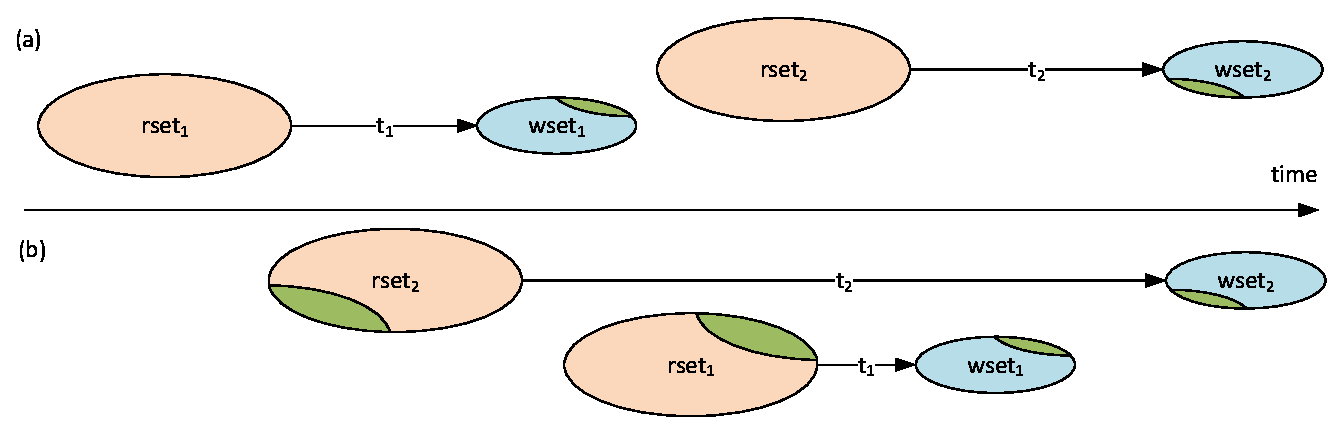
\includegraphics[width=\linewidth]{handout/img/7-ww2.eps}
    \caption{ww等价于$t_1t_2$冲突集}\label{fig:7-ww2}
\end{figure}

根据前面多版本下rr、rw、wr、ww的讨论，本讲义认为：在多版本模型下，只有一种冲突rw，甚至可以不称之为冲突，称为潜在依赖。在多版本模型下，要分析rw冲突集是否等价，在提交时刻保证新版本时戳更高。

\begin{theorem}
    一个多版本调度能够正确并发，当且仅当存在一个串行化调度，其rw冲突集等价于该多版本的冲突集。
\end{theorem}
\begin{theorem}\label{theorem:7-circle}
    多版本能够正确并发，当且仅当冲突图上无环。
\end{theorem}

\subsection{一些异常}

文献\cite{fekete2005making}认为SI的异常都是写偏write skew。写偏write skew是多版本模型下一种特殊的异常，单版本模型下没有这种异常。由于多版本模型下，常用的隔离级别就两个：SI+可串行化，写偏当然是SI级别下特有的一种异常。

写偏表现为多个事务写入不同的对象，满足SI的写入条件，但这些对象在逻辑上又是有约束的，写入会导致异常。由于表现为写入不同的对象，就象代数里的偏序，所以称为写偏。

本文对写偏并没有过分关注，它只是一种异常，理论上的判据为冲突图上是否存在环。

\begin{example}\label{ex:7-skew1}
    考虑如下一个调度，分析调度的冲突集，画出冲突图。
$$
m = r_1(x)r_2(y)w_1(y)w_2(x)
$$
$m$的冲突集为$conf(m)= \{ (r_2(y),w_1(y)),(r_1(x),w_2(x)) \}$，对应的冲突图如下：
\begin{figure}[H]
    \centering
    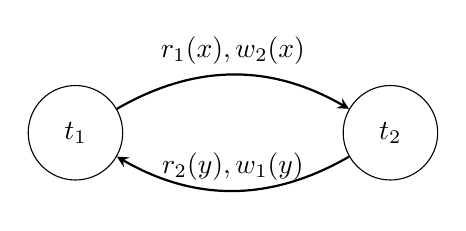
\begin{tikzpicture}[node distance=4cm, auto, >=stealth]
        % 事务节点
        \node[draw, circle, minimum size=1.2cm] (t1) {$t_1$};
        \node[draw, circle, minimum size=1.2cm, right of=t1] (t2) {$t_2$};

        % 冲突边
        \draw[->, thick] (t2) to [bend left=30] node[above] {$r_2(y),w_1(y)$} (t1);
        \draw[->, thick] (t1) to [bend left=30] node[above] {$r_1(x),w_2(x)$} (t2);
    \end{tikzpicture}
    \caption{\examplename\ref{ex:7-skew1}的冲突图}
    \label{fig:7-skew1}
\end{figure}
\end{example}

\examplename\ref{ex:7-skew1}是一个典型的写偏例子，两个事务分别读一个对象，然后分别写入另一个对象。在SI隔离级别中，这是允许的，但在可串行化隔离级别中，出现冲突环，是一个异常。

\begin{example}\label{ex:7-skew2}
    考虑如下调度，
$$
m = r_2(x)r_2(y)r_1(y)w_1(y)c_1r_3(x)r_3(y)c_3w_2(x)c_2
$$
$m$的冲突集为$conf(m) = \{ (r_2(y),w_1(y)),(r_3(x),w_2(x))\}$，对应的冲突图为：
\begin{figure}[H]
    \centering
    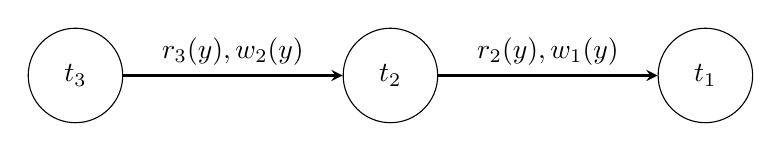
\begin{tikzpicture}[node distance=4cm, auto, >=stealth]
        % 事务节点
        \node[draw, circle, minimum size=1.2cm] (t2) {$t_2$};
        \node[draw, circle, minimum size=1.2cm, right of=t2] (t1) {$t_1$};
        \node[draw, circle, minimum size=1.2cm, left of=t2] (t3) {$t_3$};

        % 冲突边
        \draw[->, thick] (t2) to node[above] {$r_2(y),w_1(y)$} (t1);
        \draw[->, thick] (t3) to node[above] {$r_3(y),w_2(y)$} (t2);
    \end{tikzpicture}
    \caption{\examplename\ref{ex:7-skew2}的冲突图}
    \label{fig:7-skew2}
\end{figure}
冲突图上并没有环，无异常。但是，冲突图并没有表达提交，按照冲突图应该$t_2 < t_1$，实际调度中，$c_1$先提交，与冲突提示的提交顺序相悖。\figurename\ref{fig:7-skew2}中，$t_3$是一个只读事务，它不会改变异常结果，在应用中，只读事务是一个观察者，会观察到这次异常。
\end{example}

\begin{exercise}
    只读事务由于没有wset，实际可以直接省略。将\examplename\ref{ex:7-skew2}中拿掉只读事务，冲突集和冲突图是怎样的？
\end{exercise}

在组提交策略下，事务写完数据后会紧跟提交动作，在其后的读操作会读到新写入的版本，wr不被认为是冲突，原因是w对应的事务已经提交，这是两个事务的串行操作。\examplename\ref{ex:7-skew2}中，冲突意味着事务间的执行顺序，它与调度中的提交顺序是矛盾的，所以有问题。

\begin{example}\label{ex:7-skew3}
    考查如下的调度
$$
m = r_1(s)w_1(y)r_2(s)w_2(z)c_1c_2
$$
其中$s$表示一个范围，意思是$t_1, t_2$先锁住一个范围，然后分别写其中的$y, z$值，$y, z \in s$。调度对应的冲突集是$conf(m) = \{(r_2(s),w_1(y)),(r_1(s),w_2(z))\}$，因为$s \cap y, z \neq \emptyset$，所以$r_2(s),w_1(y)$、$r_1(s),w_2(z)$是冲突的。冲突集对应的冲突图如下：

\begin{figure}[H]
    \centering
    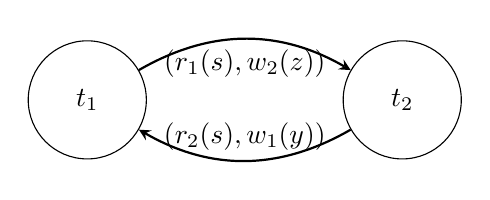
\begin{tikzpicture}[node distance=4cm, auto, >=stealth]
        % 事务节点
        \node[draw, circle, minimum size=1.5cm] (t1) {$t_1$};
        \node[draw, circle, minimum size=1.5cm, right of=t1] (t2) {$t_2$};

        % 冲突边
        \draw[->, thick] (t2) to [bend left=30] node[above, align=center] {$(r_2(s),w_1(y))$} (t1);
        \draw[->, thick] (t1) to [bend left=30] node[below, align=center] {$(r_1(s),w_2(z))$} (t2);
    \end{tikzpicture}
    \caption{\examplename\ref{ex:7-skew3}的冲突图}
    \label{fig:7-skew3}
\end{figure}

\figurename\ref{fig:7-skew3}中，存在冲突环，是一个异常。
\end{example}

\examplename\ref{ex:7-skew3}取自\cite{fekete2005making}，文献中称为谓词读锁predicate read lock，意思是以一个逻辑判断作为谓词，然后封装成锁。每次在锁表搜索时，进入该范围，都会去执行这个谓词判断。

\begin{example}\label{ex:7-skew4}
    这个例子取自\cite{berenson1995critique}，文献中称为A5A读偏read skew。考查如下的调度：
$$
m = r_1(x)w_2(x)w_2(y)c_2r_1(y)
$$
$m$的冲突集为$conf(m) = \{(r_1(x),w_2(x))\}$，对应的冲突图为：

\begin{figure}[H]
    \centering
    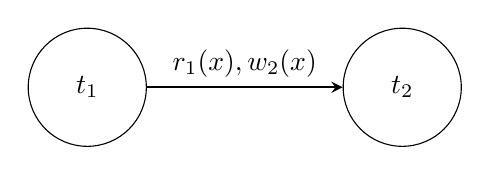
\begin{tikzpicture}[node distance=4cm, auto, >=stealth]
        % 事务节点
        \node[draw, circle, minimum size=1.5cm] (t1) {$t_1$};
        \node[draw, circle, minimum size=1.5cm, right of=t1] (t2) {$t_2$};

        % 冲突边 - 只有一个冲突
        \draw[->, thick] (t1) to node[above, align=center] {$r_1(x),w_2(x)$} (t2);
    \end{tikzpicture}
    \caption{\examplename\ref{ex:7-skew4}的冲突图}
\end{figure}

在\cite{berenson1995critique}中，$r_1(y)$会读新版本，发生读偏异常，但即使在SI隔离级别，$r_1(y)$读取的仍是旧版本，$w_2(y)$新版本对$t_1$不可见。冲突图无环，不会发生读偏，并且注意到$t_1$其实是一个只读事务。

\end{example}

\begin{example}\label{ex:7-skew5}
    这个例子取自\cite{berenson1995critique}的P4，称为lost update。考查如下调度：
$$
m=r_1(x)w_2(x)w_1(x)c_1
$$
它的冲突集为$conf(m) = \{(r_1(x),w_2(x))\}$，对应的冲突图为：

\begin{figure}[H]
    \centering
    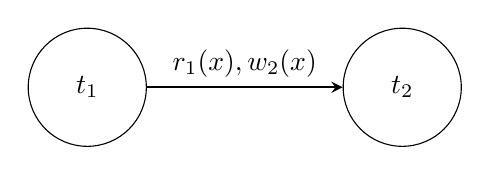
\begin{tikzpicture}[node distance=4cm, auto, >=stealth]
        % 事务节点
        \node[draw, circle, minimum size=1.5cm] (t1) {$t_1$};
        \node[draw, circle, minimum size=1.5cm, right of=t1] (t2) {$t_2$};

        % 冲突边 - 只有一个冲突
        \draw[->, thick] (t1) to node[above, align=center] {$r_1(x),w_2(x)$} (t2);
    \end{tikzpicture}
    \caption{\examplename\ref{ex:7-skew5}的冲突图}
\end{figure}

在多版本模型下，其实更新并没有丢失，只是存储为一个版本而已。冲突图无环，可串行化。但是按照$r_1(x)w_2(x)$冲突提示，$t_1$应该先提交，$w_1(x)$应该先于$w_2(x)$，出错。这个例子在本讲义的场景下稍微有点问题，按照组提交策略，$w_2(x)$后应该紧跟一个$c_2$。

\end{example}

在以上的例子中，在应用\theoremname\ref{theorem:7-circle}判定调度是否可串行化，当无环时，冲突提示了提交顺序，在提交时应该补充提交顺序的检查。

\subsection{WSI}

前述的例子中，判断调度是否可串行化，只需要检查冲突图是否存在环即可。但在工程中，有几个方面的问题，一是环的检测开销比较大，二是读集合一般都很大，冲突图会很复杂。因此工程上完整实现基于SI的可串行化存在性能上的问题，需要简化环的检测判据。

SI级别只甄别ww冲突，WSI（Write-Snapshot Isolation）\cite{cahill2009serializable}引入rw时空重叠作为冲突，在提交时检查rset、wset是否出现冲突，如果出现冲突则取消。WSI不构建冲突图，不检查图中是否存在环，它是对可串行化的判据是充分但不必要的，可能会误杀一些事务。

WSI的提交算法如下，在提交时首先检查读集合$R_r$，如果有新提交的行，则取消提交，然后更新写集合。实际上算法仍然需要象SI那样检查写集合的时戳，原算法有疏漏。同时按照WSI提交算法，只读事务可能会被取消，为避免这一点，WSI要求只读事务的读集合被清空，绕开算法，但用户必须先确定当前事务是一个只读事务。

\begin{algorithm}[H]\label{alg:wsi}
    \caption{WSI Commit ($T_s(txn_i), R_w, R_r$): \{commit, abort\}}
    \begin{algorithmic}
        \For{each row $r \in R_r$}
            \If{$\mathrm{lastCommit}(r) > T_s(txn_i)$}
                \State\Return abort;
            \EndIf
        \EndFor
        \State \Comment{Commit $txn_i$}
        \State $T_c(txn_i) \gets \mathrm{TimestampOracle.next()}$
        \For{each row $r \in R_w$}
            \State $\mathrm{lastCommit}(r) \gets T_c(txn_i)$;
        \EndFor
        \State\Return commit;
    \end{algorithmic}
\end{algorithm}

\begin{exercise}
    用WSI方案处理\examplename\ref{ex:7-skew1}。
\end{exercise}
\begin{exercise}
    用WSI方案处理\examplename\ref{ex:7-skew2}。
\end{exercise}
\begin{exercise}
    用WSI方案处理\examplename\ref{ex:7-skew3}。
\end{exercise}
\begin{exercise}
    用WSI方案处理\examplename\ref{ex:7-skew4}。
\end{exercise}
\begin{exercise}
    用WSI方案处理\examplename\ref{ex:7-skew5}。
\end{exercise}

WSI算法要求事务在本地维持一个读集合和写集合，采用组提交策略，写集合是必须维持的，并且写集合一般并不大，维持读集合就比较成问题。

\begin{figure}[H]
    \centering
    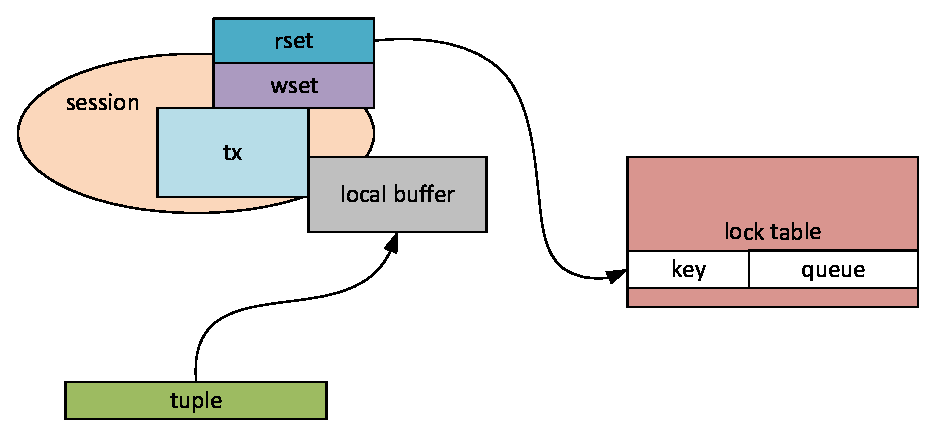
\includegraphics[width=\linewidth]{handout/img/7-rset.eps}
    \caption{读集合实现}\label{fig:7-rset}
\end{figure}

\subsubsection*{读集合}

读集合实现一般会利用锁表，读一行，会加读锁，锁进入全局锁表，每个事务自己还必须跟踪这个锁。如前所述，基于SI的方案，不会被阻塞，这个读锁也不会阻塞自己以及其它事务。这个锁不同于锁方案的锁，它的相容性矩阵不同，不会阻塞写锁。——此锁非彼锁。

在\figurename\ref{fig:7-rset}中，事务$tx$在会话中执行，它将一个tuple读到会话本地的局部缓冲，在锁表中加读锁，这个读锁的索引在事务本地以一个链表形式维持，指针指向全局锁表的表项。

在多版本模型下，读锁是加在版本上的，写锁也是加在版本上的，但是会影响上一个版本的读锁。

\subsection{SSI}

WSI方案中，只要读集合被修改，在提交时刻就无法通过rset的检查，会被取消。正如在锁方案中所了解到的，在调度中出现冲突并不可怕，冲突只是提示了事务两两之间的前后串行顺序，只要提交顺序与这个顺序一致，就不会出现问题。WSI的方案太过侵略性，损失了许多合法的调度。

SSI\cite{cahill2009serializable}与WSI相比，要精细一些，但它仍然没有完整检测环，仍然会出现误杀现象。

\begin{algorithm}[H]\label{alg:ssi}
    \caption{SSI Commit $\mathrm{commit}(T)$}
    \begin{algorithmic}[1]
        \State \textbf{atomically:}
        \State \quad \texttt{set } $T.\text{running} = \text{false}$
        \If{$T.\text{inConflict} \land T.\text{outConflict}$}
            \State \texttt{abort}$(T)$
            \State \Return UNSAFE\_ERROR
        \EndIf
        \Statex \Comment{existing SI code for $\mathrm{commit}(T)$, do not release SIREAD locks}
        \If{$T$ holds any SIREAD locks}
            \State suspend $T$, keeping SIREAD locks active
        \EndIf
        \If{$T$ was the oldest active transaction}
            \State clean up any suspended transactions older than active transactions
        \EndIf
    \end{algorithmic}
\end{algorithm}

SSI在每个事务引入两个bool变量：$T.\text{inConflict}$和$T.\text{outConflict}$，分别表示事务在冲突图上是否有入边和出边，暗示是否有环。每次事务开启，都会分配起始时戳，清掉这两个变量。

在事务提交时，SSI检查事务的$T.\text{inConflict}$和$T.\text{outConflict}$是否为真，同时为真则取消提交，意思是既有出边又有入边，说明事务在冲突图上可能有环，无法提交。这个入边出边主要是在读写操作时，根据rw冲突填写。在组提交策略下，一般是其它事务更新该事务的读集合，会产生一个出边标记，入边标记只会在短暂的提交阶段出现。

SSI的怪异之处在于第7行，事务已经提交，仍然需要维持该事务的读锁，直到与该事务的rset有交集的所有事务都提交或者取消。意思是要维持一个僵尸事务rset，用于判断是否有环。

SSI方案的出发点是利用\theoremname\ref{theorem:7-circle}，但在实际系统中，一般事务提交会释放所有锁，而rset是用读锁实现的。事务一旦提交，需要释放锁，销毁它的rset。这样一来就无从判断一个调度是否出现环，因为环上某个因果链缺失了，环被打断了。

\begin{algorithm}[H]\label{alg:ssi-write}
    \caption{SSI Write $\mathrm{write}(T, x, x\text{New})$}
    \begin{algorithmic}[1]
        \State \textbf{get lock}$(key = x,\ owner = T,\ mode = EXCLUSIVE)$
        \For{each conflicting SIREAD lock $(rl)$}
            \If{$rl.owner.running \lor \mathrm{commit}(rl.owner) > \mathrm{begin}(T)$}
                \If{$rl.owner \text{ is committed} \land rl.owner.inConflict$}
                    \State abort$(T)$
                    \State \Return UNSAFE\_ERROR
                \EndIf
                \State set $rl.owner.outConflict = \text{true}$
                \State set $T.inConflict = \text{true}$
            \EndIf
        \EndFor
        \Statex \Comment{existing SI code for $\mathrm{write}(T, x, x\text{New})$, do not get the EXCLUSIVE lock again}
    \end{algorithmic}
\end{algorithm}

SSI除了在提交时刻检查是否可能出现环，还会在wset上检查是否可能出现环。如\algorithmname\ref{alg:ssi-write}，当前事务有入边，而wset上有新版本，可能出现环。

\begin{example}
    用SSI方案处理\examplename\ref{ex:7-skew1}：
$$
m = r_1(x)r_2(y)w_1(y)c_1w_2(x)
$$
当事务$t_1$提交，只有一个入边，按照SSI提交协议\ref{alg:ssi}，$t_1$会被允许提交，同时标记$t_2$有一条出边。当$t_2$提交，写入$x$，发现$t_1$在读$x$，注意此时$t_1$已提交，因此标记为一条入边。这样，$t_2$的$\text{inConflict}$和$\text{outConflict}$都为true，回滚。
\end{example}

\begin{example}
    用SSI方案处理\examplename\ref{ex:7-skew2}：
$$
m = r_1(s)w_1(y)r_2(s)w_2(z)c_1
$$
在组提交策略下，$t_1$提交写入$y$，出现一条入边，同时标记$t_2$有一条出边。当$t_2$提交，准备写入$z$，此时$t_1$已提交，但有一个僵尸事务在维持rset，然后出现一条入边，因此$t_2$回滚。
\end{example}
\begin{example}
    用SSI方案处理\examplename\ref{ex:7-skew5}：
$$
m=r_1(x)w_2(x)c_2w_1(x)c_1
$$
按照组提交策略对原调度修改，$t_2$先提交，写入$x$新版本，事务标定入边，设定$t_1$有一条出边。当$t_1$提交，先尝试写入$x$，按照\algorithmname\ref{alg:ssi-write}，会检查$x$是否有新版本，如果有，写入新版本的事务已提交且有入边，则回滚。
\end{example}

\begin{example}\label{ex:ssi}
    SSI会导致误杀，这里构造一个用例。假设有一个公司有两张表，一张是当前的销售表，一张是按月的销售收入统计表。在下月的第1天统计上月的销售情况，更新销售收入统计表。
$$
m = r_1(x)r_2(y)w_2(x)c_2r_3(z)w_1(z)c_1
$$
在上述调度中，$t_1$对应于统计事务，$t_2$是一个更新销售表的事务，$t_3$是一个读取销售收入统计表的只读事务。$x$表示销售表的tuple，$y$表示销售收入统计表的tuple，$z$表示统计表的另一个tuple。

这个调度的冲突集是$conf(m)=\{(r_1(x),w_2(x)), (r_3(z),w_1(z)) \}$，对应的冲突图如下：

\begin{figure}[H]
    \centering
    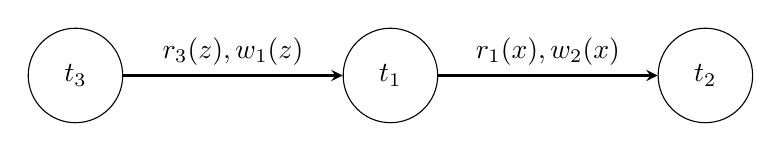
\begin{tikzpicture}[node distance=4cm, auto, >=stealth]
        % 事务节点
        \node[draw, circle, minimum size=1.2cm] (t1) {$t_1$};
        \node[draw, circle, minimum size=1.2cm, right of=t1] (t2) {$t_2$};
        \node[draw, circle, minimum size=1.2cm, left of=t1] (t3) {$t_3$};

        % 冲突边
        \draw[->, thick] (t1) to node[above, align=center] {$r_1(x),w_2(x)$} (t2);
        \draw[->, thick] (t3) to node[above, align=center] {$r_3(z),w_1(z)$} (t1);
    \end{tikzpicture}
    \caption{SSI误杀案例}
    \label{fig:ssi-false-positive}
\end{figure}

冲突图中，没有出现环，可串行化。但按照SSI算法，$t_1$提交时，会出现入边和出边，判断为可能出现环，被放弃，出现误杀。

\end{example}

\begin{exercise}
    用SSI方案处理\examplename\ref{ex:7-skew3}。
\end{exercise}
\begin{exercise}
    用SSI方案处理\examplename\ref{ex:7-skew4}。
\end{exercise}

\subsubsection*{僵尸事务}

SSI\cite{cahill2009serializable}并没有详细描述僵尸事务如何维持，基本思路参考\figurename\ref{fig:7-zombie}，$t_x$事务的起始时戳和提交时戳用于区隔，系统范围内只要存在一个事务落在这个范围内，并且与$t_x$的rset有交集，则必须保留这个僵尸事务。

在\figurename\ref{fig:7-zombie}中，$t_3$事务无需考虑，$t_1, t_2$事务完结就可以删除僵尸事务。但是，实际系统中，只要$t_1$不提交，是无从了解是否与rset有交集的。因此，僵尸事务的清理条件为，Active Transaction Table, ATT表中的启动时戳大于$t_x$的提交时戳，就可以清理$t_x$的遗留信息了。

\begin{figure}[H]
    \centering
    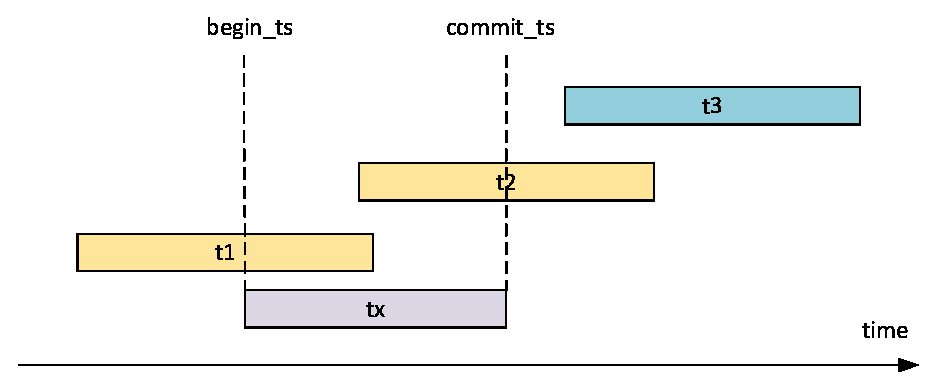
\includegraphics[width=0.8\linewidth]{handout/img/7-zombie.eps}
    \caption{僵尸事务实现}\label{fig:7-zombie}
\end{figure}

\subsection{CSI}

SSI方案通过保留僵尸事务来维持rset，用于判断是否出现环，付出的成本是维护僵尸事务，并且可能出现误杀。这里提出一种无环检测的SI可串行化方案，检测提交事务是否出现冲突环，称为CSI，unCircular SI。CSI的基本思路是，冲突并不可怕，冲突提示了事务提交的顺序，将这些提示收集为一个集合，当事务提交时，检查是否违反冲突提示即可。

\begin{figure}[H]
    \centering
    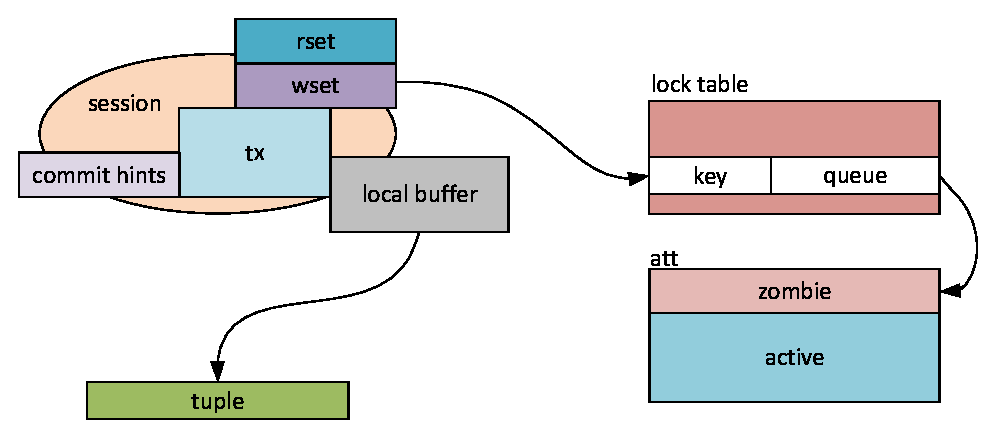
\includegraphics[width=\linewidth]{handout/img/7-csi.eps}
    \caption{CSI实现}\label{fig:7-csi}
\end{figure}

如\figurename\ref{fig:7-csi}所示，CSI在事务中增加了一个提交提示表。已提交事务在写入数据时，会产生rw冲突，这些冲突会被传递给各事务的提交提示表，该表记录了冲突图上该事务的所有出边。当该事务提交，检查wset，填写所有rset冲突事务的提交提示表，在填写时检查本地的提交提示表，如果匹配则出现环，取消写入，回滚。——此为方案一。

方案一，仍然不能避免所有环。将已提交事务之间的rw关系做剪枝，让事务指向未提交事务。——此为方案二，方案二更完整。

方案三，结合\figurename\ref{fig:7-zombie}，过滤掉所有提交时戳小于该事务的启动事务的已提交事务。

\begin{example}
    利用CSI处理\examplename\ref{ex:ssi}：
$$
m = r_1(x)r_2(y)w_2(x)c_2r_3(z)w_1(z)c_1
$$
$t_2$提交，在$t_1$的提交提示表中添加$commit\_ts(t_2)$，然后提交成功。$t_1$提交，由于更新的是$z$，在$t_3$的提交提示表中添加$commit\_ts(t_1)$。然后剪枝已提交事务的冲突图，在$t_3$的提交提示表中，添加$commit\_ts(t_2)$。
\end{example}

\section{对象的并发}

前述的单版本、多版本的并发都是基于行模型，更复杂的是对象模型。对象模型在行模型基础上，会组合成语义更复杂的上层操作，如\figurename\ref{fig:7-tree}。用户调用事务接口总是从上层开始的，这些操作最终被分解为行模型的叶子节点上的操作。考虑到各种操作可能会异步执行，\figurename\ref{fig:7-tree}的执行会以偏序森林的方式执行，对象的并发以这种偏序森林为模型展开讨论。

以一个web服务为例，一般会在服务端设置应用服务器，底层存储数据库。如果该web服务向外暴露事务接口，该接口的内部实现一般分层实现。以银行账户转账接口为例，应用服务器实现对单个账户的取款withdraw和存款deposit，取款与存款动作再分解为底层数据库行上的操作。两个转账事务$t_1, t_2$，$t_1$将钱从a账户转到b账户，$t_2$将钱从b账户转到c账户，\figurename\ref{fig:7-object}展示了这两个事务的并发执行过程。

\begin{figure}[H]
    \centering
    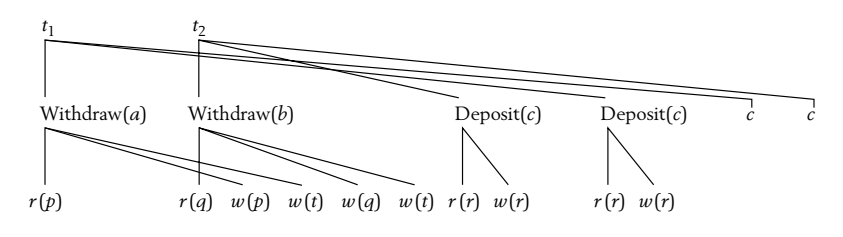
\includegraphics[width=\linewidth]{handout/img/7-object.png}
    \caption{对象并发执行}\label{fig:7-object}
\end{figure}

观察\figurename\ref{fig:7-object}，在根节点，两个事务顺序执行。但分解到取款与存储动作后，两个动作就开始并发执行。如果允许单个事务内部分层执行可以异步并发，例如存款取款并发由多个线程执行，可以想象，这种分层结构的操作构成了复杂的偏序森林。在形如\figurename\ref{fig:7-object}模型上讨论对象并发的正确性，就显得很复杂。

但实际上，对象并发性在学术届很少被讨论。对这个问题我们有几个判断：一个高层的事务接口被分解为行模型后，底层行模型的并发能保证多个事务并发的正确性。这个正确性有几个方面前提，前提一，要求单个事务并发后执行正确。一般会以一个线程对应一个用户会话，虽然理论上允许多线程并发实现高层事务，但实际系统中没这么复杂。前提二，高层事务能最终分解为行模型，这并不总是成立的，因为系统内部有一些维护程序，它们的动作也会被看成一些事务，这些维护程序并不是以行模型为叶子节点。

\section{谓词锁与锁表方案}

在前述的讲解中，我们都假设对行加锁，这简化了问题。但在实际应用中，SQL语句的WHERE子句会使用复杂的谓词限定查询范围，然后读取数据修改。如果谓词是单行，容易实现，麻烦的是范围锁如何处理。一种方案是将它们转换为行级锁，这个开销其实不小，因为需要在锁表中创建大量的行级锁。另一种方案是在采用Innodb的gap锁，对范围内所有行加锁，同时为防止幻读，对行与行间的间隙加锁。这两种方案都是基于btree，要对范围内的所有行加锁。

从上面的分析可以看到，将谓词转换为行或索引上的锁，并不是一种很好的方案。有几个方面的问题，首先要正确的将谓词转换为行上的操作；其次是行锁的粒度太小，锁表会非常大，导致锁表扫描成本过高；最后，还要防止幻读。所以，一般是直接将谓词处理为锁，称为谓词锁。

\begin{figure}[H]
    \centering
    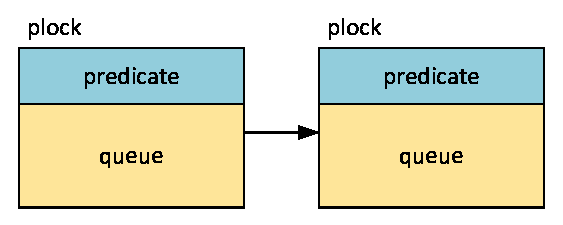
\includegraphics[width=0.6\linewidth]{handout/img/7-predicate.eps}
    \caption{谓词锁}\label{fig:7-predicate}
\end{figure}

谓词锁的实现如\figurename\ref{fig:7-predicate}所示，主要分为两部分，一部分是谓词，谓词表现为一个函数对象，范围一个bool值，当执行这个函数对象，返回true时，说明该谓词对当前行成立，对当前行加锁。另一部分是队列，用于存放等待的事务。

\figurename\ref{fig:7-predicate}中，谓词锁构成一个链表，要挨个尝试完队列中的所有谓词锁，分别确定哪些需要加锁。这个开销是比较大的，因为要遍历队列中的所有元素。

一个完整的、工程可用的锁表方案，并不容易，要容纳不同粒度的锁，如行级锁、范围谓词锁等。\figurename\ref{fig:7-predicate}将所有谓词堆砌在一起，性能不好。

mvcc的锁其实用得不多，SSI方案需要借助于锁表实现rset，在OLAP场景中，mvcc的锁表会非常大，导致锁表扫描成本过高。Neumann\cite{neumann2015fast}借助于precision lock\cite{jordan1981precision}方案，用谓词表达式来替代rset表示，而wset一般是点集，在多版本模型下，wset会自然体现为新版本。在提交验证阶段，用当前事务的wset的点去测试已提交事务的rset，同时检查rset上是否有新版本，如果有则用新版本测试提交事务的rset。

\begin{figure}[H]
    \centering
    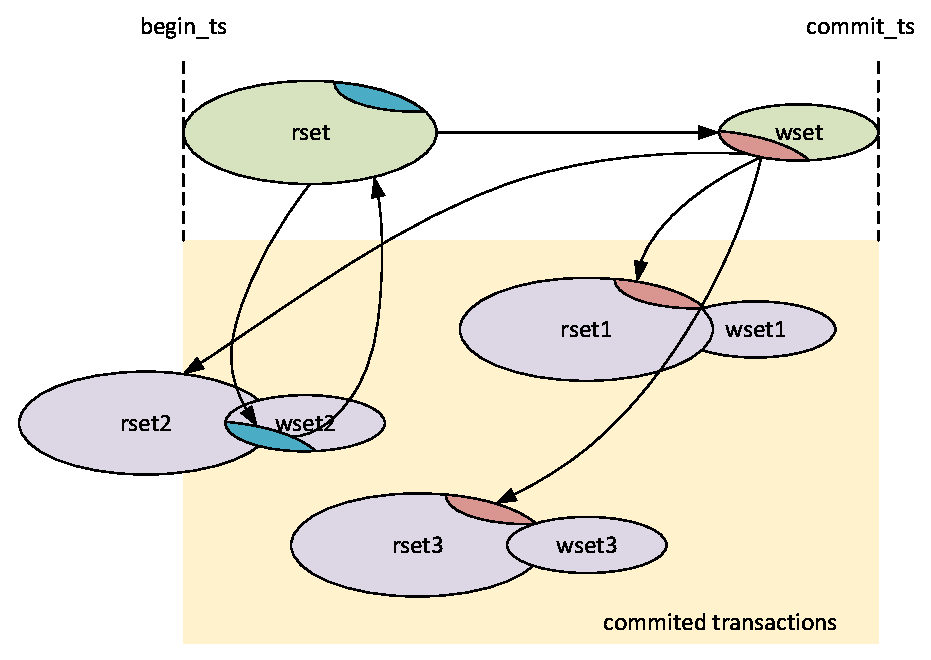
\includegraphics[width=0.8\linewidth]{handout/img/7-pt.eps}
    \caption{使用谓词锁替代rset}\label{fig:7-pt}
\end{figure}

如\figurename\ref{fig:7-pt}所示，在提交验证阶段，从两个方面验证rw冲突：1. 提交事务自己的rset用谓词表示，去rset上寻找被修改的行，找到后将这些新版本去匹配rset的谓词；2. 用当前wset上的点去测试过往已提交事务rset的谓词，找到冲突集。
